Graphs are fundamental data structures in many applications, such as computer networks, recommendation systems, and circuit design. In recent years, a number of high performance graph processing frameworks have emerged. State-of-the-art frameworks include Gunrock \cite{wang2016gunrock}, Hornet \cite{busato2018hornet}, Ligra \cite{shun2013ligra}, and Galois \cite{nguyen2013lightweight}.\ignore{These frameworks have demonstrated efficient computation on billion-scale graphs.} Their emphasis lies in accelerating graph analytics tasks by providing high-performance kernels tailored to diverse datasets.

Unfortunately, loading graph data is a significant bottleneck in such frameworks. In fact, the cost of loading data can dominate the overall processing time --- especially as computational capabilities continue to improve\ignore{\cite{gabert2021pigo}}. Gabert and Çatalyürek \cite{gabert2021pigo} observe that\ignore{even on high-performance shared-memory graph systems running billion-scale graphs,} reading the graph from file systems, on such frameworks, takes multiple orders of magnitude longer than running the computational kernel. This slowdown not only causes a disconnect for end users and a loss of productivity for researchers\ignore{/developers}, but also increases the system/cloud usage charges. Fast loading of graphs is thus, crucial\ignore{for minimizing the time it takes to start processing and analyzing the graph data}.\ignore{This motivates us to work on efficient IO techniques. These not only improve response time, but also help lower system / cloud usage charges.}

In modern frameworks like Gunrock, loading graph data from ASCII-based file formats, specifically using the Coordinate (COO) format, is a major bottleneck. To load the graph as an Edgelist, these frameworks typically follow a sequential process of opening the input file, reading the entries one by one, and inserting them into an array. If the goal is to access the graph in the Compressed Sparse Row (CSR) format, which is often the case --- due to its storage efficiency and locality benefits, additional steps are required. These include computing the out-degrees of vertices from the Edgelist, performing prefix sum to determine the offsets of outgoing edges in the CSR representation, and then populating the CSR arrays with edges from the Edgelist. All these operations are carried out sequentially, contributing to the overall loading time.

Many graph processing frameworks\ignore{have showcased efficient computation on large-scale graphs, they}, thus, still rely on sequential I/O. This is likely due to the belief that I/O devices tend to be slow (relative to the CPU), and that achieving parallel I/O necessitates specialized systems.\ignore{Graph and matrix I/O times are seldom reported in the literature.} However, modern IO devices are fast, and implementing only sequential I/O fails to exploit the capabilities of modern Hard Disk Drives (HDDs), Redundant Array of Independent Disks (RAID) controllers, and Non-Volatile Memory (NVM) \cite{gabert2021pigo}. A number of disk-based out-of-memory graph processing systems/frameworks\ignore{\cite{zhu2015gridgraph, cheng2015venus, chi2016nxgraph, ai2017squeezing, ma2017garaph, maass2017mosaic, wu2018redio, ai2018clip, jun2018grafboost, zhang2018wonderland}} \cite{kyrola2012graphchi, han2013turbograph, roy2013x, najeebullah2014bishard, lin2014mmap, zheng2015flashgraph, wang2021scaleg} focus on loading large graphs stored in binary formats. However, a majority of graph datasets exist in serialized human-readable data exchange formats.\ignore{To address this, our focus lies on efficiently loading graphs stored in plain text formats.}

To address these challenges, Gabert and Çatalyürek introduce PIGO \cite{gabert2021pigo}, a header-only, dependency-free C++11 parallel graph loader that supports loading graphs in memory as Edgelists or CSR. PIGO leverages memory mapping, a mechanism that maps a file or part of a file into the virtual memory space\ignore{so that files on the disk can be accessed as if they were in memory} \cite{lin2014mmap}, to optimize file reading. This eliminates the need for repeated system calls, resulting in reduced context-switch overhead and improved efficiency, particularly if the kernel\ignore{accurately} predicts the accessed pages ahead of time.

However, we have identified a few issues with PIGO. Firstly, when reading entries from the input file, PIGO divides the file length equally among threads, potentially leading to slower overall performance as faster threads wait for slower ones. Secondly, PIGO adopts a two-pass approach for loading graphs as Edgelists. First, it counts newlines to determine the number of edges to read, and the associated offsets to write to in the Edgelist, for each thread. Next, it parses the entries for each edge in the file and populates the Edgelist. This method is inefficient compared to a single-pass approach. To convert the Edgelist to CSR format, PIGO first computes vertex degrees globally (using atomics), uses it to compute the CSR offsets array, and then iterates through the Edgelist to atomically populate the CSR targets array. However, globally computing vertex degrees, and directly filling entries in the global CSR targets array, can lead to high contention between threads.

%% ----

% However, we have identified a few issues with PIGO. Firstly, when reading entries from the input file, PIGO divides the file length equally among threads, potentially leading to slower overall performance as faster threads wait for slower ones. Secondly, PIGO adopts a two-pass approach to load graphs as Edgelist: first, it counts the newlines to determine the number of edges to read for each thread, and then it fills in source and target vertex IDs in separate arrays in the subsequent pass, using a prefix sum to determine write offsets. This method is inefficient compared to a single-pass approach\ignore{, as discussed in our report}. To convert Edgelist to CSR format, PIGO first computes vertex degrees globally, uses it to compute offsets, and then iterates through the Edgelist to populate the CSR arrays. However, computing vertex degree globally can be inefficient due to contention between the threads. A global CSR is also directly popluated by the threads, resulting in greater contention between the threads (also the entries are populated in reverse).

% In this technical report, we propose GVEL. Similar to PIGO, it uses memory mapping along with parallelization to optimize graph loading. However, it is able to the the graph as per-thread Edgelists in a single-pass, by overallocating the needed memory through memory mapping (this does not waste memory as it, as untouched memory locations are never mapped to DRAM). Further, to convert Edgelist to CSR, GVEL computes four independent sets of vertex degrees (which, when summed up for each vertex, represent the global degree of each vertex), which it then uses to generate the global CSR representation in a novel staged manner, by first obtaining $4$ independent sets of CSRs, and then combining them together (in parallel) to form a global CSR. This minimizes the contention between threads, which we observe to be a significant bottleneck for converting an Edgelist to CSR. These allow GVEL to achieve a $2.6\times$ speedup over PIGO, in terms of Edgelist reading, and a speedup of $1.8\times$ in terms of reading the graphs as CSR (i.e., reading the graph as Edgelist and then converting it to CSR). Our techniques may also be used to convert in-memory Edgelists (an update friendly data structure), to a CSR (a space efficient and locality efficient data structure).


% Further, to populate the entries from teh Edgelist to CSR arrays, 

% While this method ensures performance, it may not be suitable for all scenarios. Finally, each thread in PIGO iterates over the degrees array to obtain start offsets, which are then used to compute the overall offsets array. Once all offsets are assigned, [...]

% However, we find a few issues with PIGO. First, for reading entries in the input file, it equally divides the length of the file between threads. This can be slow, as this would force faster threads to wait for the slower threads to complete. Second, PIGO uses a two pass approach, where it first counts the number of newlines (and thus the number of edges to read) for each thread, and in the next pass, fills in the source and target vertex IDs of the edges in two separate arrays (a prefix sum is performed to obtain the offsets, from where the threads must begin writing the source/target vertex IDs). This is inefficient, as the same can be achieved with a single pass over the file (we discuss this in this report). To convert the Edgelist to CSR format, PIGO uses a multi-pass algorithm. First, it counts the degree of each vertex, and allocates space appropriately. Next, it changes the degrees to offsets, and iterates through the Edgelist to added the entries to CSR arrays. However, it directly computes degree of each vertex, globally, with atomic operations, and static load balancing. This is for suitable for performance (DISCUSS WHY). Next, each thread in PIGO iterates over the degrees array, and obtains start offsets for each thread. This start offsets is then used to compute the overall offsets array. Once all offsets have been assigned, 

% Finally, when reading Matrix Market files, PIGO ignores the specified attributes, which causes it to report lower runtimes for symmetric graphs (the authors plan to fix this in the future).


\ignore{
%% READING PIGO CODE (CSR)
After reading a COO, they convert the COO to CSR format with \texttt{convert\_coo\_()}. Alternatively, they use \texttt{read\_graph\_()}, if the file type is specified as \texttt{GRAPH}. In \texttt{convert\_coo\_()} function, they first allocate space for the CSR. They then use a multi pass algorithm. First, they need to count each vertex's degree and allocate the space appropriately. Next, they go through the degrees and change them to offsets. Finally, they need to go through the COO and copy memory. They use plain OpenMP for, thus a static schedule with a chunk size of $1$. They atomically increment degrees, on each thread, in a global shared vector. They then do a sequential prefix sum to find the offset to write to in the offsets array (local degree count). They then do a sequential prefix sum (on the vertex range of each thread) to obtain the offsets. Their prefix sum does not start with a zero, so they adjust for this, and patch the last offset (not exactly clear to me). They then treat the degrees computed earlier as the remaining vertices, showing the current copy position. They then copy over the COO over, again an OpenMP for with static schedule of size $1$. Adding to the CSR is done with atomic capture instructions. Finally temporary arrays are freed.
}


%% TEXT BELOW NEEDS REPHRASING/SUMMARIZING

% To address these issues, Gabert and Çatalyürek \cite{gabert2021pigo} propose PIGO, a header-only dependency-free C++11 library that brings I/O improvements to graph and matrix systems. PIGO supports reading from file in parallel, with details of their secondary storage (NVMe HDD). PIGO has support for COO (coordinate-addressed matrices or graphs) and CSR (compressed sparse row matrices or graphs). However, when reading EL, they take two passes, first to count the number of newlines to determine how to allocate storage, second, copy over the values appropriately. They do not split the file into chunks, but split the file into parts, where each thread operates on its own part. They allocation is done using \texttt{std::vector::resize} (not \texttt{mmap}). When converting EL to CSR; they use plain OpenMP for, thus a static schedule; they atomically increment degrees, on each thread, in a global shared vector; They then do a sequential prefix sum (on the vertex range of each thread) to obtain the offsets. Their prefix sum does not start with a zero, so they adjust for this, and patch the last offset (not exactly clear to me). They then copy over the COO over, again an OpenMP for with static schedule of size $1$. Adding to the CSR is done with atomic capture instructions.

%% ---------------------------------------------------------------------------------------------------

% x Why do HP G frameworks load graphs slowly?
% x A quick glimpse of how they do it.
% x Why do the persist with sequential IO? (Modern IO is fast)
% x What are the HP IO interfaces? (MMAP)
% x Which graphs frameworks make use of mmap? (external memory frameworks)
% x What do they focus on? (binary graph formats)
% x Why is fast loading of serialized formats important? (human readable data exchange format)
% x What have Gabert et al. done in PIGO?
% - How do we improve upon it? (link to code)

%% ---------------------------------------------------------------------------------------------------




\ignore{Recent graph computation approaches have demonstrated that a single PC can perform efficiently on billion-scale graphs. While these approaches achieve scalability by optimizing I/O operations, they do not fully exploit the capabilities of modern hard drives and processors \cite{gualdron2016m}.}

\ignore{Many implementations persist with sequential I/O, and the article challenges the prevalent notion that parallel I/O is unattainable without dedicated systems. By exploring opportunities for parallelism through hardware RAID controllers, Non-Volatile Memory (NVM), and file system caches, the article introduces a pragmatic perspective on addressing I/O challenges. Gabert et al. present PIGO, a lightweight C++11 header-only library, as a solution that, without imposing the complexities of existing graph systems, significantly enhances end-to-end performance and productivity for researchers and developers working on shared-memory multi-core servers. Experimental results underscore PIGO's potential to redefine the landscape of optimized graph loading, complementing the strengths of popular graph processing frameworks \cite{gabert2021pigo}.}


\subsection{Our Contributions}

% This study introduces GVEL\footnote{\url{https://github.com/puzzlef/graph-csr-openmp}}, an optimized approach for reading Edgelists from text files and converting them to Compressed Sparse Row (CSR) format. GVEL outperforms Hornet, Gunrock, and PIGO in CSR reading by $78\times$, $112\times$, and $1.8\times$, respectively. With Edgelist reading, GVEL outperforms PIGO by $2.6\times$, achieving read rate of $1.9$ billion edges/s. GVEL exhibits good strong scaling, with a $1.9\times$ improvement for Edgelist reading and a $1.7\times$ increase for CSR reading with every doubling of threads.

% Our techniques may also be useful for converting COO to CSR on the fly on parallel devices. This is important since CSR is an efficient data structure, while COO is easy to update. Per-thread COOs are not needed - we can use single COO and split it unto parts for each thread to process.

% Maybe search related work on combining data to a common shared data structure. Have any others done what we have done?

% Focus on hot and cold access, and when multiple processes are accessing the same file, it can be a (significant?) advantage.

% Measure EL, CSR, EL + CSR ...
% Details of NVME, as much as possible.
% Indirect comparison with Ligra, GAPbs, and Galois (PIGO).
% Details of other graphs processing frameworks, and the above
% - cugraph
% - networkit
% - igraph?
% - gunrock
% - hornet
% - graphblast

% - adjust csr partitions
% - adjust csr partitions (convert csr only)
% - adjust block size
% - warm vs cold on graphs
% - read EL, convert CSR split on graphs



% Memory mapping is a mechanism that maps a file or part of a file into the virtual memory space, so that files on the disk can be accessed as if they were in memory \cite{lin2014mmap}. There are many advantages of using memory mapping, especially when processing large files. - Reading from and writing to a memory-mapped file do not require the data to be copied to and from a user-space buffer while standard read/write do. - Aside from any potential page faults, reading from and writing to a memory-mapped file do not incur any overhead due to context switching. - When multiple processes map the same data into memory, they can access that data simultaneously. Read-only and shared writable mappings are shared in their entirety; private writable mappings may have their not-yet-COW (copy-on-write) pages shared \cite{lin2014mmap}.




% - Why fast graph loading is important?
% - Extremely high cost of loading compared to computation.
% - An issue with even popular graph processing frameworks.
% - Modern IO is fast (compared to CPU performance).
% - Storage capacities increasing, bandwidth is high, CPUs as not as fast as they used to be.
% - Common graph file formats (COO, MTX).
% - Common memory storage formats (Edgelist, CSR).
% - Work presented in this paper.




%% - Use --- for a dash.
%% - Use ``camera-ready'' for quotes.
%% - Use {\itshape very} or \textit{very} for italicized text.
%% - Use \verb|acmart| or {\verb|acmart|} for mono-spaced text.
%% - Use \url{https://capitalizemytitle.com/} for URLs.
%% - Use {\bfseries Do not modify this document.} for important boldface details.
%% - Use \ref{fig:name} for referencing.

%% For a block of pre-formatted text: 
% \begin{verbatim}
%   \renewcommand{\shortauthors}{McCartney, et al.}
% \end{verbatim}

%% For a list of items:
% \begin{itemize}
% \item the ``ACM Reference Format'' text on the first page.
% \item the ``rights management'' text on the first page.
% \item the conference information in the page header(s).
% \end{itemize}

%% For a table:
% \begin{table}
%   \caption{Frequency of Special Characters}
%   \label{tab:freq}
%   \begin{tabular}{ccl}
%     \toprule
%     Non-English or Math&Frequency&Comments\\
%     \midrule
%     \O & 1 in 1,000& For Swedish names\\
%     $\pi$ & 1 in 5& Common in math\\
%     \$ & 4 in 5 & Used in business\\
%     $\Psi^2_1$ & 1 in 40,000& Unexplained usage\\
%   \bottomrule
% \end{tabular}
% \end{table}

%% For a full-width table:
% \begin{table*}
%   \caption{Some Typical Commands}
%   \label{tab:commands}
%   \begin{tabular}{ccl}
%     \toprule
%     Command &A Number & Comments\\
%     \midrule
%     \texttt{{\char'134}author} & 100& Author \\
%     \texttt{{\char'134}table}& 300 & For tables\\
%     \texttt{{\char'134}table*}& 400& For wider tables\\
%     \bottomrule
%   \end{tabular}
% \end{table*}


%% For inline math:
% \begin{math}
%   \lim_{n\rightarrow \infty}x=0
% \end{math},

%% For a numbered equation:
% \begin{equation}
%   \lim_{n\rightarrow \infty}x=0
% \end{equation}

%% For an unnumbered equation:
% \begin{displaymath}
%   \sum_{i=0}^{\infty} x + 1
% \end{displaymath}

%% For a figure:
% \begin{figure}[h]
%   \centering
%   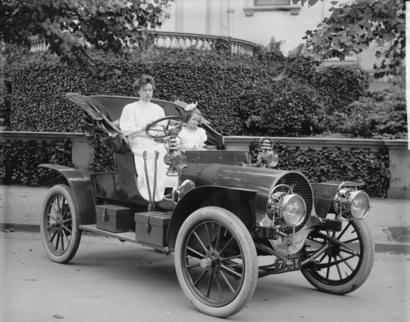
\includegraphics[width=\linewidth]{inc/sample-franklin}
%   \caption{1907 Franklin Model D roadster. Photograph by Harris \&
%     Ewing, Inc. [Public domain], via Wikimedia
%     Commons. (\url{https://goo.gl/VLCRBB}).}
%   \Description{A woman and a girl in white dresses sit in an open car.}
% \end{figure}

%% For a teaser figure.
% \begin{teaserfigure}
%   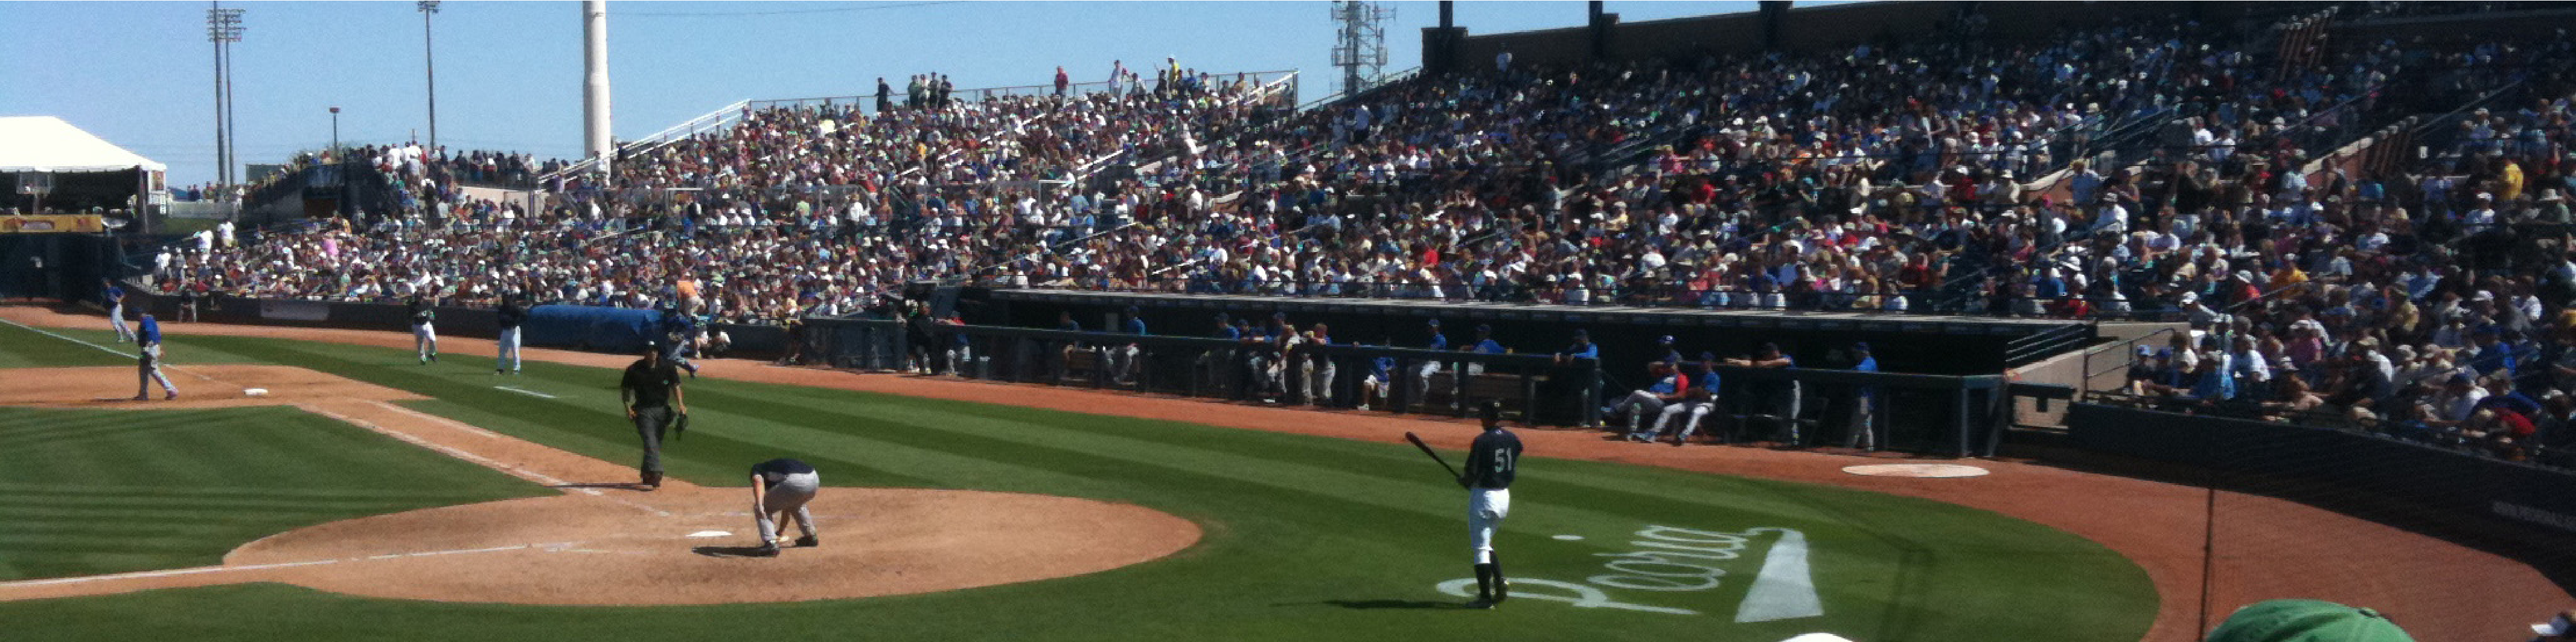
\includegraphics[width=\textwidth]{sampleteaser}
%   \caption{figure caption}
%   \Description{figure description}
% \end{teaserfigure}
